%% ===========================================================================
%%  VENUE IS UNSETTLED.  This draft is IEEEtran conference format by default,
%%  per PROTOCOL.md section 10 ("8-12 pages, IEEE or ACM two-column").  To move
%%  it to ACM, replace the two lines below with \documentclass[sigconf]{acmart}
%%  and delete \IEEEpeerreviewmaketitle; nothing else in the body depends on the
%%  class.  Every figure is drawn at 3.5in, the IEEEtran column width, so a move
%%  to acmart's 3.33in column costs a regeneration of Paper/figures and not a
%%  redraw.
%% ===========================================================================
\documentclass[conference]{IEEEtran}
\IEEEoverridecommandlockouts

\usepackage{cite}
\usepackage{amsmath,amssymb}
\usepackage{graphicx}
\usepackage{booktabs}
\usepackage{microtype}
\usepackage{url}
\usepackage{xcolor}
\usepackage[hidelinks]{hyperref}
\usepackage{balance}

%% Float placement: the paper is float-dense (five figures, six tables) and the
%% defaults leave large gaps on pages that hold one.  These loosen the limits so
%% floats and text share pages instead of alternating.
\renewcommand{\topfraction}{0.92}
\renewcommand{\bottomfraction}{0.75}
\renewcommand{\textfraction}{0.06}
\renewcommand{\floatpagefraction}{0.80}
\setlength{\textfloatsep}{8pt plus 2pt minus 3pt}
\setlength{\floatsep}{7pt plus 2pt minus 2pt}
\setlength{\intextsep}{7pt plus 2pt minus 2pt}

\newcommand{\netsanity}{\textsf{netsanity}}
\newcommand{\nmapsn}{\texttt{nmap -sn}}
\newcommand{\Refuted}{\textbf{refuted}}
\newcommand{\NotRefuted}{not refuted}
\newcommand{\qhigh}{q_{\mathrm{high}}}
\newcommand{\qlow}{q_{\mathrm{low}}}

\begin{document}

\title{Retransmit Early, Declare Late: Decoupled Timing Budgets\\for Host
Discovery on Heterogeneous Local Networks\\
\large A pre-registered measurement study, two of whose four hypotheses
its own data refutes}

\author{\IEEEauthorblockN{Juan Carlos Est\'evez Rodr\'iguez}
\IEEEauthorblockA{\textit{Independent}\\
\texttt{netsanity} --- \url{https://github.com/JCTec/netsanity}}}

\maketitle

\begin{abstract}
Host discovery on a local segment is not a throughput problem. A /24 is 254
addresses and the wire is idle at any plausible probe rate; the binding
constraint is how long a scanner waits for its slowest device before declaring
the rest absent. We describe a sweep that answers \emph{when do I resend} and
\emph{when do I give up} with two separate budgets rather than one, and report
a pre-registered measurement study of what that buys against \nmapsn{} swept
across four timing templates at two privilege levels: 1{,}580 runs over ten
days in 120 randomised interleaved blocks against a programmable
ten-responder segment spanning 1\,ms to 500\,ms of round-trip time, under a
protocol frozen before the first measurement, with three ground-truth oracles
and a passive capture per run. Two exclusions, 0.13\%.
%
Discovery completes in a median 0.382\,s against 4.31\,s for the fastest
\nmapsn{} configuration matching its recall --- an eleven-fold difference with
complete distributional separation --- and the frontier of nmap's eight
configurations collapses to a single non-dominated point.
%
\textbf{Two of the four tested hypotheses are refuted by their own
pre-declared conditions, and the abstract is where the protocol requires that
to be said.} H6 predicted that losing root costs \nmapsn{} at least 0.25 more
recall than it costs us; the measured gap is 0.10 warm and $-0.20$ cold, so H6
is refuted in both arms even though the difference is overwhelmingly
significant ($p=2\times10^{-57}$). H5 predicted that splitting the budgets
costs no recall; it holds warm and fails cold, where recall drops from 1.00 to
0.80. The mechanism is one measured fact: our shipped declaration budget
expires at about 370\,ms and the segment's slowest responders answer at
508\,ms, so replies reaching the wire inside the process's own lifetime are
never attributed. The warm arm, which carries 1{,}458 of the 1{,}580 runs,
hides this because the kernel neighbour table supplies the two hosts the sweep
did not hear.
%
Scope, which belongs here and not only in a limitations section: one hardware
model, one macOS build, one /24, one RTT dispersion, a virtual segment with no
Wi-Fi and no correlated loss, local-segment scanning only, IPv4 only, and a
cold arm of 122 runs in which no two conditions ever share a block. Nothing
here supports a claim about enterprise networks, IPv6, routed scanning or
Linux.
\end{abstract}

\begin{IEEEkeywords}
host discovery, network scanning, adaptive timing, retransmission, measurement
study, pre-registration, reproducibility, macOS
\end{IEEEkeywords}

\section{Introduction}

``Our scanner is faster than nmap'' is not a reviewable claim. Compared as
shipped, \netsanity{} performs host discovery \emph{and} three naming
protocols while \nmapsn{} performs host discovery only; a wall-clock comparison
of the two measures different work. This paper is organised around narrower
claims that can fail, and two of them do.

The technical starting point is where a local sweep spends its time. On a
consumer /24 the live host count $h$ is small and the dead count $N-h$ large
--- the development network gave $h=9$, $N-h=245$. Under a single fixed
per-attempt budget $T$ every dead address pays $k\!\cdot\!T$, because every
attempt runs to timeout, and $T$ must exceed a high quantile $\qhigh$ of the
segment's round-trip times or slow hosts are lost: \emph{every dead address
pays the slowest host's tail, $k$ times}. That is the consequence of using one
number to answer two questions. Separating them is cheap --- resending early
costs one duplicate packet, so $r$ can be driven by a \emph{low} quantile
$\qlow$, while declaring absence needs the tail but is asked once, at the end,
overlapping every address. The split is sound only if a reply arriving after
its own attempt's window has closed is still attributed to the probe that
caused it. That attribution requirement is the mechanism this paper
contributes; the budget split is its consequence, and
Section~\ref{sec:results} shows it failing on the segment we built.

\paragraph*{Contributions} A pre-registered protocol with falsification
conditions fixed before collection, four dated amendments, one withdrawn
hypothesis, and a published record from which every number here is recomputable
(Section~\ref{sec:method}). The first measurement of this technique's
speed/completeness frontier against a swept comparator (Fig.~\ref{fig:pareto}):
0.382\,s against 4.31\,s at matched recall, Cliff's $\delta=-1.000$ against
every nmap configuration, and the finding that seven of nmap's eight
configurations are dominated by the eighth. \textbf{Two refutations}: H5, that
splitting the budgets costs no recall, fails in the cold-cache arm; H6, that
losing root costs nmap more recall than it costs us, fails in both arms,
because nmap's best unprivileged template is not a better scanner but a slower
one. A mechanism for both, read off the record: a declaration budget shorter
than the segment's tail, and a warm arm whose recall is supplied by a kernel
cache the experiment's own block structure fills (Fig.~\ref{fig:budget}). A
measurement pricing the contribution against its own ablation. And the
privileged engine this study caused to be built, which appears in future work
and in no result (Section~\ref{sec:future}).

\begin{figure}[tb]
\centering
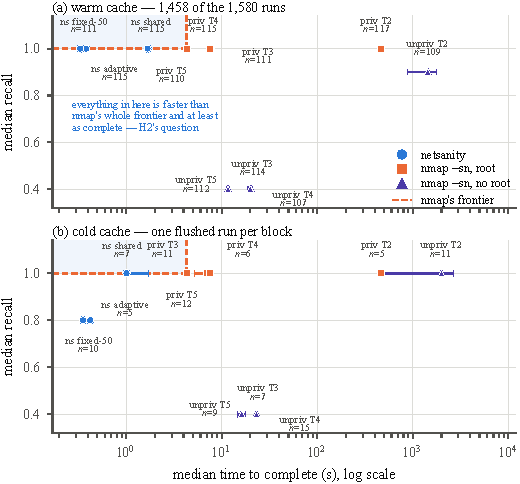
\includegraphics[width=\columnwidth]{figures/fig1_pareto}
\caption{\textbf{Every point on nmap's frontier is beaten by a \netsanity{}
configuration warm, and the configuration that beats it cold is the ablation
that turns the contributed technique off.} Speed against completeness for all
eleven discovery conditions in both cache arms; medians with bootstrap 95\%
intervals at 10{,}000 resamples, $n$ on every point. Of nmap's eight
configurations exactly one is non-dominated in either arm --- privileged
\texttt{-T5} --- so the timing sweep that was in the protocol to make the
comparison fair produces one competitor and seven dominated points. Warm, all
three \netsanity{} configurations sit inside the shaded quadrant; cold, only
the shared-budget ablation does, and the adaptive default this paper is about
sits at recall 0.80 and loses to \texttt{-T5} outright
(Section~\ref{sec:h2}).}
\label{fig:pareto}
\end{figure}

\paragraph*{A declared conflict of interest}
\label{sec:intro-coi}
We wrote one of the two systems
and chose its defaults. The protocol, harness, raw data and analysis are
published so a reviewer can rerun them, and the falsification conditions frozen
before collection are what make the declaration mean anything. Where a choice
during the study made a hypothesis easier to survive,
Section~\ref{sec:method} names the choice, its measured cost, and who made it.

\section{Background and related work}

\textbf{Retransmission timing.} Jacobson's smoothed-RTT and mean-deviation
estimator and the Karn--Partridge ambiguity rule are the canonical treatment of
\emph{when do I resend} \cite{jacobson1988,karn1987}; we apply the estimator to
discovery probing rather than to a connection. Karn's rule is
\emph{unnecessary} under per-transmission tokens, since the ambiguity it
resolves does not arise --- a claim this study does not test.

\textbf{Scale, and why its techniques do not transfer downward.} ZMap and
masscan are stateless and optimise send rate at a constant timeout
\cite{zmap2013,masscan}, which is right when the address space is enormous and
per-host state unaffordable. Local discovery inverts both assumptions: the
space is tiny and per-host state nearly free, which is what makes per-host
adaptation available to us and not to them. nmap's
\texttt{-T0}\,\ldots\,\texttt{-T5} are a discrete set of points on the
single-budget curve, chosen before the network is observed \cite{nmapbook}. Our
claim is that adaptation dominates the whole set, not that any one template is
badly chosen, which is why the comparator is swept across four templates at
each privilege level rather than left on its default.

\textbf{Timers, concurrency, naming and method.} Timing wheels make expiry
management $O(1)$ \cite{varghese1987}, which matters once each probe carries
its own deadline rather than sharing a global one; Little's Law fixes
concurrency as $c=\rho L$ rather than leaving it a tuning constant, and
bounding in-flight work bounds the latency tail
\cite{grosvenor2015,marinos2014}. mDNS/DNS-SD, SSDP and NBSTAT are prior art we
consume rather than extend \cite{rfc6762,rfc6763,upnp}, and MAC randomisation
is now the common case \cite{martin2017}, which is why identity is keyed on an
equivalence class over identifiers of differing stability rather than on the
hardware address; neither carries a timing claim. Pre-registration is standard
practice where the experimenter has a stake in the outcome \cite{nosek2018},
and a scanner benchmark published by the scanner's author is such a case.

\section{The system}
\label{sec:system}

\netsanity{} is a macOS scanner written in Swift with no subprocesses and no
external binaries. The study measures version 0.4.0 at commit
\texttt{ad09ed1}, tagged \texttt{study/bi\-nary-2026-09-12b}, built
\texttt{swift build -c release} with Apple Swift 6.3.3 for
\texttt{arm64-apple-macosx26.0}.

\subsection{The measurement model}
Let $A$ be the address set probed, $N=|A|$, $H\subseteq A$ the hosts present
and reachable in the observation window, $h=|H|$; for host $i$, $R_i$ is its
response latency with CDF $F_i$ and $\ell_i$ its per-probe loss probability, so
a probe with budget $b$ elicits a usable reply with probability
$p_i(b)=(1-\ell_i)F_i(b)$. A sweep is characterised by the attempts per address
$k$, the concurrency $c$, and either one budget $T$ or the pair $(r,t)$. In the
dead-dominated regime,
\begin{equation}
T_{\mathrm{shared}} \approx \frac{(N-h)\,k\,T}{c},\qquad T \gtrsim \qhigh
\label{eq:shared}
\end{equation}
\begin{equation}
T_{\mathrm{split}} \approx \frac{(N-h)\,k\,\qlow}{c} + t,\qquad t \gtrsim \qhigh
\label{eq:split}
\end{equation}

\subsection{What the model got wrong before any data existed}
\label{sec:sim}
A mechanism-level simulator was written from the probe/wait/resend/declare loop
--- deliberately not from Eqs.~\ref{eq:shared}--\ref{eq:split} --- and run
before the testbed was built. It refuted three parts of the model; a second,
tested simulator later withdrew two of those three refutations. Three
corrections stand and they bound what this paper may claim.

\emph{The continuous form fails at /24 scale.} With $Nk\approx762$ probes and
$c=240$ a sweep is three to five \emph{waves}, not a flow: the fixed policy
takes $\lceil Nk/c\rceil T$ to within a microsecond on 97.7\% of simulated
rows, where Eqs.~\ref{eq:shared}--\ref{eq:split} predict 0\% and run 30.6\%
low, and the split policy's counterpart is $(\lceil Nk/c\rceil-1)r+t$, one
interval shorter because once the last probe is away only the declaration
window remains.

\emph{The speedup is not the dispersion ratio, and it saturates.} With
$W=\lceil Nk/c\rceil$ and $d=\qhigh/\qlow$,
\begin{equation}
\mathrm{speedup}=\frac{Wd}{W-1+d},
\label{eq:speedup}
\end{equation}
whose largest deviation from the simulated median over dispersions of
1--80$\times$ is $0.0000$. The asymptote is the wave count, not the dispersion:
a reader applying the original ``advantage equals $\qhigh/\qlow$'' claim to a
40$\times$ network and expecting 40$\times$ will be disappointed by a factor of
nine. Raising $W$ raises the ceiling: swept from /24 to /16 at constant density and
concurrency the same configuration goes from 3.20$\times$ to 11.74$\times$.

\emph{Correlated loss is where the technique is paid for.} Against a two-state
loss process at the same marginal rate, the split policy packs three
transmissions into roughly 150\,ms so any longer outage takes all three, while
the fixed policy spreads them over $3T\approx1.9$\,s and usually straddles it:
simulated recall at a one-second mean outage is 0.855 against 0.910. The repair
is to buy the extra spacing out of the tail budget's own slack, free where that
budget is a floor. None of this is evidence about \netsanity{} --- it is
evidence about the model, whose value is that it refuted three magnitude claims
in an afternoon rather than after seven days of collection, all three in the
direction that flattered us.

\subsection{The enabling condition}
\label{sec:enabling}
The split is sound only if a reply arriving after its own attempt's window has
closed is still attributed to the probe that caused it. Otherwise shortening
$r$ turns slow hosts into missed hosts and the technique degenerates into ``use
a shorter timeout''. Two requirements follow. Each transmission carries a
unique token, so a late reply is attributable to the exact attempt it answers
--- sequence-number reuse breaks this, and at /16 scale a 16-bit field wraps
and attribution becomes silently wrong, which is worse than losing it. And an
expired probe stays in the pending table \emph{until the declaration budget
expires, not until its own window does}. The second is what this study
falsifies in its cold arm: if the declaration budget expires before the
segment's tail there is no window in which a late reply can be matched, and the
first requirement buys nothing (Section~\ref{sec:budget}).

\subsection{The platform surface}
Three macOS facts shape the design and none generalise.
\texttt{socket(AF\_INET, SOCK\_DGRAM, IP\-PROTO\_ICMP)} succeeds for an
ordinary user, so full host discovery needs no root, where a scanner assuming
raw sockets must escalate or fall back to TCP connect probes against two ports
--- a strictly weaker signal, since a host may answer ICMP and no TCP port. The
Local Network permission returns \emph{zero results rather than an error} when
denied and cannot be queried, so a denied run is exit~0, a well-formed artifact
and an empty address set; recording that as recall~0 would publish a fabricated
number, which is why the harness asserts the grant per run with a positive
control. And \texttt{/dev/bpf} nodes are exclusive-open, so a capture ---
including this study's own oracle --- can deny a privileged engine the resource
it needs.

\subsection{What does not exist, and why it matters here}
\label{sec:noengine}
\netsanity{} has no privileged engine. \texttt{EngineKind} declares
\texttt{privilegedBPF} and \texttt{composite} and neither is constructed
anywhere in the product; \texttt{ICMPSweepEngine} is the only
\texttt{HostDiscovery} conformance on Darwin and reports
\texttt{kind:\,.unprivileged} unconditionally. This was measured before it was
read: the same binary under \texttt{sudo} and as the owner, each under its own
capture with the neighbour table flushed first, is indistinguishable on the
wire --- 253 ARP requests and 20 ICMP echoes against 253 and 19, no TCP in
either, the same nine hosts. The ARP in both is the kernel resolving next-hop
for the ICMP datagrams, which is why the counts match: one engine, run twice.
Hence H3's withdrawal (Section~\ref{sec:family}); and hence the engine's
declared capabilities, \texttt{["icmp\_sweep", "neigh\-bor\_table"]}, which
name the neighbour table as a discovery source and are the mechanism behind the
warm arm's recall (Section~\ref{sec:cache}).

\section{Method}
\label{sec:method}

The protocol was frozen and dated before the first measurement run; every
change after it is an amendment with a date and a reason, and all four are
disclosed below. That discipline is the only reason the two refutations in this
paper are worth reading.

\subsection{The hypothesis family, and what happened to it}
\label{sec:family}

Five hypotheses were frozen; four are tested.
\textbf{H1 (speed, matched workload).} For host discovery alone on a
heterogeneous /24, \netsanity{}'s median time-to-complete is lower than
\nmapsn{} at every timing template achieving equal or better recall.
\emph{Refuted if} any template matches its recall at equal or lower median
time.
\textbf{H2 (the trade curve).} Per-host adaptive retransmission timing
dominates fixed timing templates on a network whose round-trip times span
orders of magnitude. \emph{Refuted if} the Pareto frontier of nmap's templates
contains a point \netsanity{} does not match or beat. This is the central
claim; H1 is a corollary.
\textbf{H4 (identification).} Fusion of mDNS, SSDP, NetBIOS and OUI data names
a larger fraction of hosts than nmap's OS fingerprinting identifies.
\emph{A capability comparison, no test, no timing claim.}
\textbf{H5 (budget separation).} Separating the retransmission budget from the
absence-declaration budget reduces total sweep time without reducing recall,
relative to a single shared budget. \emph{Refuted if} recall drops, or if the
reduction is within run-to-run noise.
\textbf{H6 (the privilege gap is nmap's).} On a local segment, losing root
costs \nmapsn{} substantially more recall than it costs \netsanity{}.
\emph{Refuted if} the median per-block recall of unprivileged \nmapsn{} --- at
its best timing template --- is less than \textbf{0.25} below unprivileged
\netsanity{}'s on the pre-declared testbed composition, or if the difference is
not significant under McNemar after Bonferroni correction.

\paragraph*{H3 was withdrawn, 2026-09-12} H3 asked whether unprivileged
\netsanity{} matches privileged \netsanity{}. Section~\ref{sec:noengine} is why
it cannot be asked: both arms execute identical code, so the claim is confirmed
on every block regardless of what the network does --- a tautology with a
$p$-value beside it. The ordering is checkable and it matters. The harness
already refused a privileged artifact reporting the unprivileged engine and
would have refused every one of them: one condition in fourteen excluded on
every block, 7.1\% against the protocol's own 5\% ceiling, before any
excluded-for-cause run. The protocol says a study above 5\% is re-designed
rather than patched; the condition was removed because it measures nothing, and
the exclusion rate went to zero as a consequence rather than as a goal.

\paragraph*{Why 0.25, and how H6's condition can fire} ``nmap is worse'' is not
falsifiable. The threshold has to be a number the data can fall short of, tied
to a composition declared in advance, because the size of the gap is a property
of what is on the segment: all web servers would give a gap near zero, all
ICMP-only hosts a gap near one. The 2026-09-08 amendment therefore pre-declared
the composition --- \emph{at least a quarter of the responders answer ICMP and
serve port 80 or 443}, beside the ICMP-filtered and TCP-only hosts already
required --- and derived 0.25 from a predicted gap near 0.75.
Section~\ref{sec:h6} reports 0.10. The same amendment fixes H6's scope: its
mechanism is ARP, which does not cross a router, so H6 is a local-segment claim
and the abstract says so.

\paragraph*{Bonferroni} The family size changed twice and both changes are
recorded rather than inferred from a count of surviving hypotheses: four at
freezing, five when H6 was added, four again when H3 was withdrawn. Every
$p$-value is corrected against four, so $\alpha_{\mathrm{Bonf}}=0.0125$.

\subsection{The testbed}
\label{sec:testbed}

The primary testbed is a \emph{programmable} segment, not a physical one
(amendment of 2026-09-06): the central claim is that the advantage scales with
RTT dispersion, and a physical network supplies whatever dispersion its
hardware happens to have --- one or two points on a curve the study needs the
whole of, and no way to reach a dispersion of~1 where the technique should show
no advantage at all. The physical home LAN became the secondary
external-validity testbed and, as Section~\ref{sec:threats} says plainly, was
never used for collection.

\begin{table}[tb]
\caption{The programmable segment, from the manifest at the final rebuild ---
two responders at each of five round-trip times. Three of ten answer ICMP and
serve a web port, against the quarter H6's amendment pre-declared. Achieved
times are measured medians over 40 probes; the study reads the achieved column,
never the target.}
\label{tab:testbed}
\centering
\footnotesize
\setlength{\tabcolsep}{3.4pt}
\begin{tabular}{@{}llrll@{}}
\toprule
 & addr. & target & achieved (ms) & roles\\
\midrule
r01, r02 & \texttt{.4, .5}   & 1\,ms   & 0.930, 0.959   & ICMP+:80; ICMP\\
r03, r04 & \texttt{.6, .7}   & 5\,ms   & 4.977, 4.988   & ICMP+:443; ICMP\\
r05, r06 & \texttt{.8, .9}   & 25\,ms  & 24.921, 24.978 & ICMP+:80,:443;\\
         &                   &         &                & \quad filtered+:80\\
r07, r08 & \texttt{.10, .11} & 100\,ms & 99.990, 99.434 & ICMP; silent (ARP)\\
r09, r10 & \texttt{.12, .13} & 500\,ms & 507.918, 506.628 & ICMP; ICMP+15\% loss\\
\bottomrule
\end{tabular}
\end{table}


Table~\ref{tab:testbed} is the bill of materials: ten responders at
\texttt{192.168.64.4}--\texttt{.13} on a \texttt{vmnet} segment reached through
\texttt{bridge100}, each a network device in its own Linux namespace inside one
of five Ubuntu virtual machines, with \texttt{netem} on its egress. Delay is
imposed \emph{at the host that answers}, which is what a genuinely slow device
does and needs no root on the scanning Mac.

Two facts had to be measured rather than assumed. The guests must be kept out
of deep idle: idle, the round trip has a median of 0.87\,ms and a standard
deviation of 1.0\,ms, against 0.33\,ms and 0.4 with one core held busy, so the
idle-exit path alone exceeds the smallest delay the segment imposes. And
open-loop shaping overshoots by $+16\%$ at a 1\,ms target, so configuration
closes the loop until the measured median is within 2\% of target; every later
stage reads the achieved column. The gate --- ten addresses, five delays, each
within 10\% of configuration on three consecutive runs, distinct hardware
addresses --- was met, and re-met on H6's composition at a worst error of
2.50\%. The segment does not survive a host reboot and was rebuilt eight times
during collection (Section~\ref{sec:repro}); at every rebuild its identity
fields are \emph{identical} and only the achieved column moves.
\textbf{Its weakest point:} at a 1\,ms target the standard deviation
across probes is 0.5--1.3\,ms, so the segment sets a responder's \emph{typical}
latency and not every probe's, and the dispersion reported here is computed
from measured medians, so its denominator is the noisy end.

\subsection{Three oracles}
\label{sec:oracles}

Recall is meaningless without knowing what was there, so three independent
views are used together and a run whose oracles disagree is excluded and the
exclusion reported. \emph{The manifest} declares what was deliberately placed.
\emph{The guests' own inventory}, read out of band, is a view of who is present
that neither scanner produced. \emph{A passive capture} --- \texttt{tcpdump} on
\texttt{bridge100}, one pcap per run, started before the process and stopped
after it --- is read post hoc for which addresses emitted or answered anything
inside the run window. The third is the only one that distinguishes ``the
scanner missed it'' from ``it was not answering'' and is therefore the one that
decides recall; in the pilot it also detected a deliberately injected link
failure that both other oracles missed. The oracle gate is three consecutive
rounds in which all three report the same ten addresses, re-run after every
rebuild.

\textbf{Recall is computed against the manifest's declared responder set and
not against what either tool returned.} Every run also found
\texttt{192.168.64.1}, the bridge the scanning Mac speaks through: a real host
and not a declared responder, so it is precision and not recall, and it puts a
ceiling of $10/11=0.909$ on the precision of every condition that reports it
(Section~\ref{sec:precision}).

\subsection{Harness independence, and the wall clock}
\label{sec:independence}

The apparatus does not share code with the thing measured. The harness is
Python and deliberately not Swift: a harness sharing code with \netsanity{} can
share a bug with it. The rule is asserted rather than claimed --- a self-check
parses every harness module with \texttt{ast} and fails if any \texttt{Import}
node names the product or its toolchain. A second rule separates the study's
halves: \textbf{the harness never computes a statistic and the analysis never
touches the network.} They meet only at an append-only NDJSON file, one line
per run, validated on write and on read, and no number in the paper may exist
that cannot be recomputed from it (Section~\ref{sec:notinrecord} reports where
this study does not meet that). The harness fails loudly rather than skipping a
condition: a dirty tree aborts the block before it starts, untracked files
included, and a refused \texttt{sudo -n}, a failed capture or a host that slept
for over a second stops the block rather than excluding one run --- if root is
not arranged, every privileged run in every remaining block fails identically.

\paragraph*{Why wall clock is taken around the process} Both tools report their
own timing and neither report is the measurement. Wall clock is taken with
\texttt{time.monotonic()} in the harness, bracketing \texttt{fork} to
\texttt{wait}, and that is the only place a duration is produced. A self-report
measures a different interval from the one a user experiences --- process
spawn, dynamic linking, the artifact write and \netsanity{}'s history write sit
inside the harness's bracket and outside the tool's own --- and taking one
would make the comparison unauditable in the direction that matters, since the
system under test was written by the authors. The schema enforces this: every
record carries \texttt{wall\_clock\_source:\,"harness\_mo\-no\-tonic"}, its
duration must fit inside the timestamps bracketing it, and the tools' own
numbers live under \texttt{tool\_self\_reported\_seconds}, a name chosen so no
analysis can reach for it by mistake; eleven adversarial mutations of a real
record were all rejected by the validator. The two clocks agree to a median
8--20\,ms per condition, worst case 0.20\,s on a 49-minute run.

\paragraph*{One departure from measuring the product as shipped}
\texttt{netsanity scan} persists every run and \nmapsn{} persists nothing, so
as shipped the conditions are not matched on I/O --- and the mismatch is not
constant: the history store rewrites itself past a line threshold, so one run
in $N$ pays for a compaction \emph{inside the measured wall clock}, on a
schedule no covariate records and in the direction that weakens H1. Every
\netsanity{} condition therefore names its own disposable store through an
explicit \texttt{env} assignment in the argv, one store per run, so every run's
write is the same constant work. This is a scanner's discovery time, not a
product's. The \texttt{env} prefix costs one extra \texttt{exec} nmap does not
pay, on the order of a millisecond, biasing H1 \emph{against} \netsanity{}.

\subsection{Design}
\label{sec:design}


Thirteen conditions ran. \netsanity{}: \texttt{scan --discovery-only} (the
adaptive default, serving H1, H2, H5, H6), the same with
\texttt{--retransmit-timeout 50ms} (the fixed ablation, H2) and with
\texttt{--shared-budget} (H5), and the full pipeline \texttt{scan} (H4). nmap:
\texttt{-sn -T2}\,\ldots\,\texttt{-T5} under \texttt{sudo} (H1, H2) and as the
owner (H1, H2, H6), and \texttt{-sn --script broadcast-*} (H4). Every nmap
invocation carries \texttt{--reason}, so the discovery reason distinguishes the
privileged and unprivileged conditions from the evidence rather than from the
command line. \texttt{ns.disc.priv} was withdrawn with H3.

\emph{Interleaved, randomised, blocked.} One block is one run of every
condition in an order randomised within the block --- never all of one tool
then all of the other, because network drift and thermal state would confound
the comparison. \emph{Stratified.} Thirty complete blocks in each of four
six-hour time-of-day strata across at least seven consecutive days, so device
sleep cycles and household load are sampled rather than avoided; the driver
caps a stratum at five blocks a day, because thirty blocks in one afternoon is
a different experiment with the same block count. \emph{Cache state is a
condition, not an accident:} the neighbour table hugely advantages any scanner
that runs second, so each block begins with a flush and warm versus cold is
analysed as two results rather than adjusted away. \emph{Cooldown: 10\,s,}
measured --- holding the capture open thirty seconds past each process's exit
showed the longest scan-attributable traffic tail to be 6.1\,s, and it belongs
to the scanning host's kernel retrying ARP for the 244 addresses that do not
answer. The cooldown stops one run's \emph{traffic} reaching the next; it does
nothing about neighbour-table state, and no cooldown short enough to run 120
blocks in a week would.

\paragraph*{The cache-state amendment of 2026-09-13, and its declared cost}
One flush before thirteen conditions makes exactly one run per block cold: 2.3
cold runs per condition per stratum against 27.7 warm, 9.2 against 110.8
pooled. The pilot made the consequence visible --- cold, the adaptive default
missed the two 500\,ms responders on fourteen of fourteen runs and found them
on eleven of eleven warm ones --- so three alternatives were costed: flushing
before every run in half the blocks (16.2 cold against 13.8 warm per stratum,
neither arm at 30, 72 machine hours against 61); holding both arms at 30 per
stratum (240 blocks, 143 machine hours, the seven-day floor moving to twelve
days); and dropping the cold arm. The first design was retained. Every option
that strengthened the cold arm also made H2, H5 and H6 easier to refute, and
the person choosing wrote the system under test. The amendment records that and
commits the study in advance to three things: the cold arm is analysed
\emph{pooled} at about nine runs per condition, every number from it carries
its $n$, and \emph{a refutation there is reported in the abstract and not in a
limitations section}. Section~\ref{sec:h5} is that refutation.

\subsection{Analysis plan, fixed in advance}
\label{sec:plan}

Medians and interquartile ranges, never means alone: scan-time distributions
are right-skewed and heavy-tailed and a mean flatters whichever system has
fewer catastrophic runs. Mann--Whitney $U$, two-sided, $\alpha=0.05$, with
Cliff's $\delta$ and Bonferroni correction across the family; bootstrap
intervals at 10{,}000 resamples; McNemar on paired per-host outcomes within a
block. H2 is answered by the speed/recall Pareto frontier with a region of
interest of $\mathrm{recall}\ge0.95$, which the simulator's C5 correction
requires be stated before the frontier rather than after it. Pre-specified
exclusions: oracle disagreement, an interfering process, a topology change ---
with the rule that an exclusion rate above 5\% means the study is re-designed
rather than patched.

\paragraph*{Amendments made during analysis} Five, all dated 2026-09-22, all
exploratory, none admitted to the family and none reading a threshold: a
Kruskal--Wallis across the strata, which the plan names no test for; a Gaussian
kernel density on $\log_{10}$ wall clock, to describe each distribution's shape
before its median is reported; unpaired bootstrap intervals on cold-arm recall
differences, because the pre-declared McNemar has nothing to pair there
(Section~\ref{sec:h5}); the adaptive default against its own fixed-retransmit
ablation, the only measurement that prices the contribution; and Jaccard set
stability. No threshold was moved, no statistic was chosen after seeing which
one flattered, and the two exclusions in the file are the two exclusions.

\section{Results}
\label{sec:results}

\subsection{What the record holds, and whether it reconciles}
\label{sec:record}

Collection ran 2026-09-13 18:19 to 2026-09-22 00:14 local (UTC$-$06:00):
\textbf{120 complete blocks, 30 in each of four strata, across ten distinct
days} against a seven-day floor, \textbf{1{,}580 records}, all schema~2,
\textbf{two exclusions, both \texttt{host\_asleep}: 0.13\% against a 5\%
ceiling}. The two blocks those exclusions stopped are partial and no census
counts them. Thirteen conditions at 120--122 runs each; \textbf{1{,}458 warm
and 122 cold}, 9.4 cold per condition, range 5--15.

An independent script recomputes every claim in the reproducibility record from
the NDJSON. \textbf{All twenty-six reconcile}: one \netsanity{} and one nmap
\texttt{sha256} across the window, \texttt{git\_dirty} false, oracles
\texttt{agree}, captures \texttt{ok} and the Local Network permission
\texttt{granted} on all 1{,}580 runs, the cooldown 10\,s on every run, and all
4{,}740 referenced stdout, stderr and capture paths present on disk.

Two rows read twice. \texttt{on\_ac\_power} is \texttt{true} on every record
\emph{including the thirty-nine runs of three blocks that ran on battery},
because the harness collects provenance once per block and copies it onto every
run; the evidence is \texttt{pmset -g log}, which is not a study artifact
(Section~\ref{sec:sensitivity}). And \texttt{host\_asleep\_seconds} exceeds
zero on 148 runs, 146 of them between 1\,ms and 75\,ms --- clock skew rather
than sleep --- and the two above the one-second threshold are the two
exclusions.

\paragraph*{The stratum hole, and how it was closed} \textbf{No record stores
its stratum, and none carries a timezone or UTC offset.} The driver bucketed a
naive local hour, so a reader in another timezone re-derives identical
per-stratum counts with every block relabelled and nothing anywhere firing. The
offset was established from artifacts: the driver's 120 ``block finished'' log
lines, read as UTC and subtracted from the epoch time of the last record of the
block each closes, give \textbf{$-21{,}600$\,s on all 120 anchors}, write lag
1.517--2.669\,s, total spread across the window 1.152\,s --- no drift, no
daylight-saving step --- and all seven apparatus commits independently carry a
$-0600$ committer offset. A derived sidecar reproduces the driver's own labels
for all 122 blocks with zero disagreements and leaves \texttt{runs.ndjson}
untouched.

\paragraph*{Which apparatus each block ran under} Seven commits appear in one
contiguous sweep with no interleaving (65, 192, 221, 413, 78, 598 and 13 runs).
\textbf{None changed the measurement path}: no diff between consecutive commits
touches the product, the harness or the analysis, and the frozen packages diff
empty against the binary tag at all seven. Across all seven rebuilds the
testbed's identity fields are identical and only the achieved column moves, so
there is no between-block confound in what the testbed \emph{is}. One rebuild
calibrated at 7.00\% worst error against 1.22--1.60\% for the other six,
covering block 121 alone. \textbf{It stays}, for four reasons: the error is
inside the 10\% tolerance fixed before any data existed and the oracle gate was
met after it; the absolute miss is 70\,$\mu$s on a 1\,ms responder and 8\,ms on
a 500\,ms one, where the study's fastest condition has an 8\,ms interquartile
range; all thirteen runs sit inside their own conditions' distributions, the
most extreme at the 94th percentile; and removing it would take the overnight
stratum below the protocol's own floor on a ground the protocol does not name.

\subsection{Every distribution, before any median}
\label{sec:shapes}

\begin{figure}[tb]
\centering
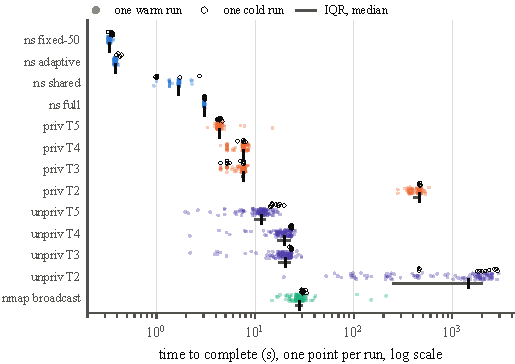
\includegraphics[width=\columnwidth]{figures/fig2_distributions}
\caption{Every \netsanity{} condition is tight and single-peaked and every nmap
condition is not: coefficients of variation run 0.004--0.104 for \netsanity{}
against 0.11--0.73 for nmap, and unprivileged \texttt{-T2} is filled
continuously across two orders of magnitude rather than being bimodal. A median
describes the top four rows and describes nothing about the twelfth.}
\label{fig:dists}
\end{figure}

Figure~\ref{fig:dists} is every run in the study and
Table~\ref{tab:conditions_summary} every median. Four conditions need prose.

\textbf{Unprivileged \texttt{-T2} is the one whose median describes nothing.}
Warm, $n=109$: median 1{,}446\,s, IQR 245--2{,}030\,s, full range
19.5--2{,}947\,s, $p_{90}/p_{10}=23.5$. A kernel density on $\log_{10}$ wall
clock finds humps near 250\,s and 1{,}900\,s, but the valley between them is
97\% as tall as the lower peak: not two clean modes, a distribution
continuously filled across two orders of magnitude. It is reported as a
distribution and never as a median.

What separates its runs is in the record and it is not nmap. \textbf{Its wall
clock rank-correlates with the number of ARP requests the scanning host's
kernel emitted at $\rho=+0.972$} over 109 warm runs (Fig.~\ref{fig:arp}) --- a
count ranging from 0 to 2{,}387 for the same binary, argv and segment, on runs
whose exit status is 0 and whose parse succeeded. It carries recall with it:
recall rank-correlates with wall clock at $+0.787$ and with the TCP RST count
at $+0.900$, because the longer the kernel keeps it waiting the more
closed-port resets it is still listening for. Its 37 warm runs at recall 0.40
have a median wall clock of 217\,s; its 52 at recall 1.00, 2{,}060\,s.
\textbf{Unprivileged \texttt{-T2} does not have a recall; it has a recall as a
function of how long the scanning host's kernel made it wait} --- the single
most important caveat on H6.

\textbf{Unprivileged \texttt{-T3}, \texttt{-T4} and \texttt{-T5} each have a
small fast mode} --- six to twenty runs between 2.0 and 9.0\,s against a main
mode at 12--23\,s --- explained by the same covariate: those runs emitted
0--87 ARP requests instead of 500--770. Their recall does not move with it:
0.40 in 107 of 107 \texttt{-T4} and 112 of 112 \texttt{-T5} warm runs.
\textbf{Privileged \texttt{-T3} and \texttt{-T4} are genuinely multimodal at a
small scale} --- 16\% of runs near 5.2\,s against a main mode near 7.6\,s ---
so their medians are reported with an IQR beside them and not alone.
\texttt{ns full} at $CV=0.004$ is the most reproducible measurement here.

\paragraph*{Precision inverts, for a reason that is not about correctness}
\label{sec:precision}
Median precision is 0.909 for all four \netsanity{} conditions and all four
privileged nmap templates, and 1.000 for all four unprivileged templates and
the broadcast condition. \textbf{Nothing found a false positive in 1{,}578
runs}: every address any condition reported was a declared responder or the
bridge. The unprivileged templates score higher only because they find four
hosts instead of eleven and never see the bridge. Without that sentence beside
it, the precision column says the opposite of what happened.

\begin{table}[tb]
\caption{Median time to complete, with the interquartile range, and median
per-block recall, by cache arm. \emph{Read the cold column with its $n$:} one
flush per block gives each condition five to fifteen cold runs in 120 blocks.}
\label{tab:conditions_summary}
\centering
%% generated by Paper/scripts/make_tables.py from Study/data/runs.ndjson -- do not edit
\scriptsize
\setlength{\tabcolsep}{2.6pt}
\begin{tabular}{@{}lrlcrlc@{}}
\toprule
& \multicolumn{3}{c}{warm arm} & \multicolumn{3}{c}{cold arm}\\
\cmidrule(lr){2-4}\cmidrule(lr){5-7}
condition & $n$ & median (s) & rec. & $n$ & median (s) & rec.\\
\midrule
\texttt{ns fixed-50} & 111 & 0.331\,{\tiny[0.327--0.335]} & 1.00 & 10 & 0.354\,{\tiny[0.346--0.361]} & 0.80 \\
\texttt{ns adaptive} & 115 & 0.382\,{\tiny[0.377--0.386]} & 1.00 & 5 & 0.422\,{\tiny[0.412--0.427]} & 0.80 \\
\texttt{ns shared} & 115 & 1.681\,{\tiny[1.673--1.690]} & 1.00 & 7 & 1.011\,{\tiny[1.003--1.365]} & 1.00 \\
\texttt{ns full} & 112 & 3.054\,{\tiny[3.049--3.063]} & 1.00 & 10 & 3.083\,{\tiny[3.078--3.089]} & 0.80 \\
\texttt{priv T5} & 110 & 4.308\,{\tiny[4.242--4.328]} & 1.00 & 12 & 4.320\,{\tiny[4.271--4.425]} & 1.00 \\
\texttt{priv T4} & 115 & 7.592\,{\tiny[7.549--7.710]} & 1.00 & 6 & 7.622\,{\tiny[7.591--7.693]} & 1.00 \\
\texttt{priv T3} & 111 & 7.684\,{\tiny[7.232--7.812]} & 1.00 & 11 & 7.079\,{\tiny[5.205--7.642]} & 1.00 \\
\texttt{priv T2} & 117 & 466.4\,{\tiny[405.0--470.0]} & 1.00 & 5 & 467.9\,{\tiny[464.9--471.5]} & 1.00 \\
\texttt{unpriv T5} & 112 & 11.67\,{\tiny[9.905--12.66]} & 0.40 & 9 & 16.21\,{\tiny[14.66--17.32]} & 0.40 \\
\texttt{unpriv T4} & 107 & 19.94\,{\tiny[17.03--22.59]} & 0.40 & 15 & 23.17\,{\tiny[23.06--23.31]} & 0.40 \\
\texttt{unpriv T3} & 114 & 20.30\,{\tiny[17.44--22.56]} & 0.40 & 7 & 23.18\,{\tiny[23.07--23.25]} & 0.40 \\
\texttt{unpriv T2} & 109 & 1,446.0\,{\tiny[244.5--2,030.0]} & 0.90 & 11 & 2,001.5\,{\tiny[1,124.0--2,507.5]} & 1.00 \\
\texttt{nmap broadcast} & 108 & 28.12\,{\tiny[25.83--30.29]} & 0.40 & 14 & 30.25\,{\tiny[29.96--30.60]} & 0.40 \\
\bottomrule
\end{tabular}

\end{table}

\subsection{H1 --- speed at matched recall}
\label{sec:h1}

\textbf{Warm: refutation condition not met --- \NotRefuted{}.} The adaptive
default runs in a median \textbf{0.382\,s} (IQR 0.377--0.386, bootstrap 95\%
interval on the median [0.380, 0.383], $n=115$) at median recall 1.00. Four
templates match that recall, all privileged: \texttt{-T2} at 466.4\,s,
\texttt{-T3} at 7.68\,s, \texttt{-T4} at 7.59\,s, \texttt{-T5} at 4.31\,s.
\textbf{The fastest is 11.3 times slower.} Every pairwise Mann--Whitney $U$ is
$p\le2.2\times10^{-38}$ with Cliff's $\delta=-1.000$ --- complete separation,
no \netsanity{} run overlapping any nmap run --- and every bootstrap interval
on the median difference excludes zero by orders of magnitude.

\textbf{Cold: refutation condition not met --- \NotRefuted{}, $n=5$.} The
default runs in 0.422\,s at median recall 0.80. Five templates match or beat it
--- privileged \texttt{-T2}--\texttt{T5} and unprivileged \texttt{-T2}, all at
1.00 --- and the fastest is privileged \texttt{-T5} at 4.32\,s, ten times
slower. $\delta=-1.000$ against each; $p$ ranges $3.2\times10^{-4}$ to
$7.9\times10^{-3}$, and against $\alpha_{\mathrm{Bonf}}=0.0125$ the privileged
\texttt{-T2} comparison at $p=0.0079$ is the only one not comfortably clear of
it. Here H1 survives \emph{because \netsanity{} is fast, not because it is
complete}: it wins on time while losing on recall, which the refutation
condition permits by construction and which a reader should be told plainly.

\subsection{H2 --- the trade curve, and the result to argue about}
\label{sec:h2}

The first thing the frontier shows is about nmap. \textbf{Of the eight
\texttt{-sn} configurations exactly one is non-dominated, in both arms:
privileged \texttt{-T5}}, at 4.308\,s and recall 1.00 warm ($n=110$) and
4.320\,s and 1.00 cold ($n=12$). Every other configuration is slower at the
same or lower recall; \texttt{-T3} and \texttt{-T4} are indistinguishable from
each other. Sweeping \texttt{-T2}--\texttt{T5} was in the protocol so that
comparing against \texttt{-T3} alone could not be called dishonest; on this
testbed it produces one competitor and seven dominated points.

\textbf{Warm: refutation condition not met --- \NotRefuted{}.} All three
\netsanity{} discovery configurations beat privileged \texttt{-T5}:
fixed-retransmit 0.331\,s, adaptive default 0.382\,s, shared budget 1.681\,s,
all at median recall 1.00 against 4.308\,s. The adaptive default alone beats
it, so the verdict does not depend on how ``a \netsanity{} configuration'' is
read, and under the region of interest ($\mathrm{recall}\ge0.95$) the same
single nmap point qualifies and the same three beat it.

\textbf{Cold: refutation condition not met as written --- and this is the
result to argue about.} The literal condition asks whether \emph{some}
\netsanity{} configuration is faster than privileged \texttt{-T5} and at least
as complete. One is: \textbf{the shared-budget ablation}, at 1.011\,s and
recall 1.00 on $n=7$ against \texttt{-T5} at 4.320\,s and 1.00 on $n=12$. But
the cache-state amendment names a narrower clause and commits the paper to the
abstract if it fires: \emph{``if the cold arm shows a privileged nmap point at
recall 1.0 that \netsanity{} does not match\,\ldots{} H2 is reported as refuted
in the cold regime and the paper says so in the abstract.''} Read as the
adaptive default, cold median recall is 0.80 against four privileged points at
1.0 and the clause \textbf{fires}; read as any configuration in the matrix it
is 1.00 and it does not.

\textbf{The judgement, as a judgement rather than a computation.} H2's headline
attributes the domination to \emph{per-host adaptive retransmission timing},
and the configuration that rescues it cold is the shared budget --- the one
that does \emph{not} use the technique this paper contributes, and the one H5
exists to argue against. Reporting H2 as surviving the cold arm on the strength
of its own null ablation would be making a claim its reader should not accept.
So both are reported: the pre-declared condition is not met, in those words,
and the amendment's clause fires on the claim the paper is actually making.
Either way the cold arm's resolution is five observations of the default and
seven of the shared budget.

\subsection{H5 --- the budget split, refuted in the cold arm}
\label{sec:h5}

\textbf{Warm: refutation condition not met --- \NotRefuted{}.} Split budget
0.382\,s (IQR 0.377--0.386, $n=115$) against shared 1.681\,s (IQR
1.673--1.690, $n=115$): a \textbf{4.40-fold reduction}, median difference
$-1.2986$\,s, bootstrap interval $[-1.3022,-1.2966]$, excluding zero by three
orders of magnitude, so the reduction is not within run-to-run noise. Recall
1.00 against 1.00, and McNemar over 108 paired blocks and 1{,}080 paired host
observations finds \textbf{zero discordant pairs in either direction}.

\textbf{Cold: refutation condition met --- \Refuted{}, $n=5$ and 7.} Split
0.422\,s against shared 1.011\,s --- the reduction is still there and still
outside noise (median difference $-0.590$\,s, $[-1.308,-0.566]$, $p=0.0025$)
--- but \textbf{recall drops, from the shared budget's 1.00 to the split
budget's 0.80}. The first disjunct of H5's refutation condition is exactly
``recall drops'', and it does.

\textbf{The pre-declared test cannot be run here, and the reason is
structural.} The plan pairs per-host outcomes \emph{within a block}, and one
flush per block makes exactly one run per block cold, so \textbf{no two
conditions are ever cold in the same block and the cold arm contains zero
within-block pairs for any pair of conditions} --- which also removes the
paired test under H6. The amendment reasoned about the cold arm's $n$ and did
not notice it had removed the pairing. The verdict does not depend on it, since
``recall drops'' is read off recall, but the significance machinery the
protocol specified is unavailable in the arm where the refutation happens. The
unpaired bootstrap interval on the median recall difference is
$-0.200\ [-0.200,-0.200]$, reported as the exploratory substitute it is.

\subsection{H6 --- the privilege gap, refuted in both arms}
\label{sec:h6}

\begin{figure}[tb]
\centering
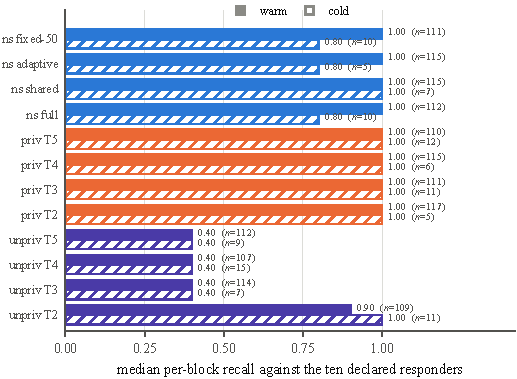
\includegraphics[width=\columnwidth]{figures/fig3_recall_by_cache}
\caption{\textbf{The privilege gap H6 predicted is 0.10 warm and $-0.20$ cold
against a pre-declared 0.25, so H6 is refuted in both arms --- and the template
that refutes it is not a better scanner but a slower one.} \texttt{-T3},
\texttt{-T4} and \texttt{-T5} behave exactly as the mechanism predicts, at 0.40
in 321 of 333 warm runs; \texttt{-T2} reaches 0.90 warm and 1.00 cold by
running for a median 24 minutes and collecting closed-port resets while it
waits.}
\label{fig:recall}
\end{figure}

Figure~\ref{fig:recall} is the recall of every condition in both arms.

\textbf{Warm: refutation condition met --- \Refuted{}.} The best unprivileged
template by median per-block recall is \texttt{-T2} at \textbf{0.90};
\texttt{-T3}, \texttt{-T4} and \texttt{-T5} are all at 0.40. Unprivileged
\netsanity{} is at 1.00. \textbf{The gap is 0.10 against a pre-declared 0.25},
so the first disjunct fires and H6 is refuted on it alone; the unpaired
bootstrap interval on the median difference is $0.100\ [0.000,0.200]$, whose
upper end does not reach 0.25 either. The second disjunct does not fire:
McNemar over 104 paired blocks and 1{,}040 paired host observations gives
\textbf{257 hosts found only by \netsanity{} against 0 found only by nmap,
$p=2.1\times10^{-57}$}, far below $\alpha_{\mathrm{Bonf}}$.

\textbf{Cold: refutation condition met --- \Refuted{}, $n=5$ and 11.}
Unprivileged \texttt{-T2} reaches a median per-block recall of \textbf{1.00}
against \netsanity{}'s 0.80. The gap is $\mathbf{-0.20}$ and the first disjunct
fires; the second cannot be evaluated, for the reason given under H5.

\textbf{Why the gap is not what the amendment predicted, and it is not because
the mechanism is wrong.} \texttt{-T3}, \texttt{-T4} and \texttt{-T5} behave
exactly as the pre-collection characterisation said unprivileged nmap would:
recall 0.40 in 321 of 333 warm runs, recovering only the three web hosts and
the TCP-only host, by \texttt{syn-ack}. The gap against \netsanity{} there is
0.60 and H6's threshold would have cleared comfortably. What defeats H6 is
\texttt{-T2}, which is not a better scanner but a slower one: the kernel's ARP
retry behaviour keeps it running for a median 1{,}446\,s and up to 2{,}947\,s,
and while it runs it collects TCP RSTs from closed ports on hosts answering no
probed service, which nmap counts as up by \texttt{conn-refused}. Fifty-two of
its 109 warm runs reach recall 1.00 and thirty-seven sit at 0.40, and which one
a block gets is set by the scanning host's kernel. So: \textbf{``at its best
timing template'' turned out to select a template whose recall is a function of
the measurement environment.} The amendment derived 0.25 from a composition
that was right and a prediction that was not, because nobody predicted
\texttt{-T2} would be allowed to run for three quarters of an hour. That is a
defect in the prediction, not the threshold, and moving the threshold now is
what the analysis plan forbids. Table~\ref{tab:verdicts} collects the four
verdicts.

\begin{table}[tb]
\caption{The four verdicts, against conditions frozen before collection.}
\label{tab:verdicts}
\centering
\footnotesize
\begin{tabular}{@{}lll@{}}
\toprule
 & warm arm & cold arm\\
\midrule
H1 & \NotRefuted{} & \NotRefuted{} ($n=5$ vs 5--15)\\
H2 & \NotRefuted{} & not refuted as written; the amendment's\\
   &               & \quad clause fires for the default ($n=5$)\\
H5 & \NotRefuted{} & \Refuted{} --- recall $1.00\!\to\!0.80$\\
H6 & \Refuted{} --- gap 0.10 & \Refuted{} --- gap $-0.20$\\
\bottomrule
\end{tabular}
\end{table}

\subsection{The mechanism: a declaration budget shorter than the tail}
\label{sec:budget}

\begin{figure}[tb]
\centering
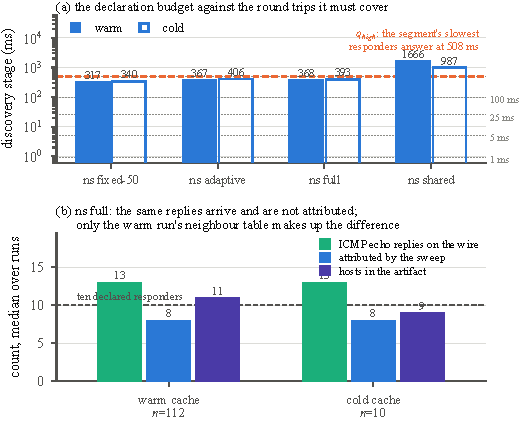
\includegraphics[width=\columnwidth]{figures/fig4_declaration_budget}
\caption{\textbf{The shipped declaration budget expires before the segment's
slowest host answers, and the replies that arrive inside the process's own
lifetime are never attributed.} (a) Every split-budget configuration's
discovery stage closes at 317--406\,ms against responders measured at 508\,ms;
only the shared-budget ablation, at 987--1{,}666\,ms, outlives the tail it must
cover. (b) For the one condition whose process outlives that tail sixfold, the
capture records the same thirteen echo replies warm and cold and the sweep
attributes eight in both --- yet the artifact reports eleven hosts warm and
nine cold.}
\label{fig:budget}
\end{figure}

This is the finding the rest of the cold-arm results follow from, and it is
entirely in-record; Table~\ref{tab:budget} is the evidence. The segment's
slowest responders are configured at 500\,ms and measured between 497 and
508\,ms at every rebuild, and Eq.~\ref{eq:split} requires $t\gtrsim\qhigh$.
\textbf{The split budget's whole discovery stage is 317 to 406\,ms --- shorter
than $\qhigh$ alone, before any of the sweep.} The shared budget's is 987 to
1{,}666\,ms and it never misses a host in 122 runs. Every cold miss in the
study is the same two addresses: \texttt{192.168.64.12} and \texttt{.13}, the
two 500\,ms responders, account for \textbf{every} missed host --- 24 and 23
occurrences --- and \textbf{no other address is ever missed by \netsanity{}
anywhere in the collection.}

\begin{table}[tb]
\caption{The declaration budget, read off the record. \emph{echo wire} is ICMP
echo replies in the run's own capture, \emph{attr.}\ what the discovery stage
attributed, \emph{rep.}\ what the artifact reported, \emph{slow} how many of
the two 500\,ms responders were found on average. Warm runs put \emph{zero} ARP
replies on the wire and still report both slow hosts: the neighbour table
already held them.}
\label{tab:budget}
\centering
%% generated by Paper/scripts/make_tables.py from Study/data/runs.ndjson -- do not edit
\scriptsize
\setlength{\tabcolsep}{2.6pt}
\begin{tabular}{@{}llrrrrrrrr@{}}
\toprule
condition & arm & $n$ & stage & echo & ARP & attr. & rep. & slow & rec.\\
 & & & (ms) & wire & repl. & & & /2 &\\
\midrule
\texttt{ns fixed-50} & warm & 111 & 317 & 13 & 0 & 8 & 11 & 1.98 & 1.00 \\
 & cold & 10 & 340 & 8 & 10 & 9 & 9 & 0.10 & 0.80 \\
\addlinespace[1.5pt]
\texttt{ns adaptive} & warm & 115 & 367 & 13 & 0 & 8 & 11 & 2.00 & 1.00 \\
 & cold & 5 & 406 & 7 & 12 & 8 & 9 & 0.00 & 0.80 \\
\addlinespace[1.5pt]
\texttt{ns full} & warm & 112 & 368 & 13 & 0 & 8 & 11 & 2.00 & 1.00 \\
 & cold & 10 & 393 & 13 & 11 & 8 & 9 & 0.40 & 0.80 \\
\addlinespace[1.5pt]
\texttt{ns shared} & warm & 115 & 1,666 & 12 & 0 & 13 & 11 & 2.00 & 1.00 \\
 & cold & 7 & 987 & 12 & 11 & 7 & 11 & 2.00 & 1.00 \\
\bottomrule
\end{tabular}

\end{table}

\subsection{The warm arm measures a cache, not a sweep}
\label{sec:cache}

The discovery stage's reply and host counts were added to the record precisely
so this could be checked from the file. \textbf{The adaptive default attributes
a median of eight replies warm and eight cold --- the same number --- and
reports eleven hosts warm against nine cold.} The two extra hosts warm are not
something it heard: the block's flush empties the neighbour table and the
previous run in the block fills it.

The cleanest evidence is the full-pipeline condition's cold runs, clean because
that process lives 3.08\,s --- over six times the slowest round trip --- so its
capture is a fair witness where a 0.35\,s process's is not. \textbf{Those runs
put 12 to 13 ICMP echo replies on the wire inside the process's own lifetime;
the discovery stage, which closed at 393\,ms, attributed eight, and the
artifact reported nine hosts in seven of ten runs and ten in two more.} The
replies arrived, inside the process, inside the capture, and were not
attributed.

Table~\ref{tab:budget} settles what the warm arm measured. \textbf{Warm runs of
every \netsanity{} condition put zero ARP replies on the wire} --- the kernel
had no address to resolve --- \textbf{and found both 500\,ms responders anyway,
2.00 of 2.00.} Cold runs put 10 to 12 ARP replies on the wire and found 0.00 to
0.40 of them, except the shared budget, whose 987\,ms stage outlives the tail
and which found 2.00 of 2.00 cold as well. So the warm arm's recall of 1.00 is
the neighbour table the block structure filled, and the shared budget's cold
1.00 is the only \netsanity{} recall in the study a sweep earned on a flushed
cache.

This contradicts Section~\ref{sec:enabling} directly. \textbf{The prediction
that recall is invariant to the budget split, given per-transmission tokens and
matchable expired probes, is contradicted in the cold arm}, at 0.80 against
1.00. The theory says a recall drop here means straggler attribution is broken
rather than that the technique is wrong, and the measurement agrees:
per-transmission identity buys nothing when the pending table is emptied before
the tail arrives. The warm arm does not rescue this --- it hides it, in
1{,}458 of 1{,}580 runs.

\subsection{Adaptation costs time and buys nothing measurable here}
\label{sec:ablation}

The matrix contains \netsanity{}'s own fixed-50\,ms-retransmit ablation, which
keeps the budget split and removes the per-host adaptation. No hypothesis asks
for the comparison; it is the only thing in the study that prices the mechanism
the paper contributes. Warm, it runs in 0.331\,s ($n=111$) against the adaptive
default's 0.382\,s ($n=115$): median difference $-50.9$\,ms $[-52.4,-48.6]$,
$\delta=-1.000$, $p=1.4\times10^{-38}$. Cold, 0.354\,s ($n=10$) against
0.422\,s ($n=5$): $-67.6$\,ms $[-87.6,-39.1]$, $\delta=-1.000$,
$p=6.7\times10^{-4}$. \textbf{Complete separation: no adaptive run is faster
than any fixed-retransmit run, in either arm.} Recall is indistinguishable ---
1.00 against 1.00 warm, McNemar over 105 paired blocks and 1{,}050 paired host
observations finding two observations recovered only by the adaptive default
against none the other way ($p=0.5$, exact binomial), and 0.80 against 0.80
cold. \textbf{Adaptation costs 13\% of the sweep warm and 16\% cold and returns
nothing this testbed can measure} --- on a testbed holding one dispersion and
constant per-responder latency, which is the regime where a fixed interval
tuned to the segment should do well.

\subsection{Where the measurements contradict the simulation}
\label{sec:vs-sim}

The simulator of Section~\ref{sec:sim} predates the testbed and is evidence
about the model. Four places where the two disagree, and in all four
\textbf{the measurements win}.

\textbf{Straggler attribution never failed in simulation, and fails here.} Of
1{,}140 missed hosts in a 2{,}000-replicate simulation at five declaration
budgets, \emph{all} were categorised \texttt{all\_transmissions\_lost} and
\emph{none} had a reply arriving after the last matchable instant; the paired
recall difference between the split and shared policies was exactly zero in
every one of 2{,}000 replicates at every budget. The measurement is the
opposite: 12--13 replies on the wire, 8 attributed, a 0.20 recall difference
cold. The simulator could not see it because \emph{it took $t$ as a parameter};
the shipped system derives $t$ from the replies it has seen, so on a segment
where the fast hosts answer first the tail is never sampled and $t$ lands below
$\qhigh$ by construction. A model in which $t$ is given cannot express a system
in which $t$ is estimated.

\textbf{The failure mode the simulation predicted is not the one that
happened.} The simulator's strongest warning was that the split policy loses
recall under \emph{correlated} loss --- nine recall points at a one-second
outage --- because it packs its transmissions into a window shorter than a
typical outage. This segment has no burst process at all, and the split policy
loses 20 recall points anyway, for an unrelated reason.

\textbf{The speedup law is the right shape and the wrong constant here.}
Equation~\ref{eq:speedup} with $W=\lceil 254\cdot3/240\rceil=4$ and a measured
dispersion $d=508/0.93=546$ predicts a split-versus-shared speedup of
$3.98\times$. The measurement is $\mathbf{4.40\times}$ warm
($1.681/0.382$), 11\% high; inverting the law on the measured speedup gives an
effective $W\approx4.4$. Direction and order of magnitude survive, the constant
does not, and \emph{the record cannot settle it}: $c$, $r$ and $t$ are not in
the schema (Section~\ref{sec:notinrecord}).

\textbf{The comparator does not trace a monotone frontier.} The model assumed
nmap's templates trace a monotone speed/recall curve along which adaptation
must lie strictly below-right; seven of eight are dominated by the eighth
(Section~\ref{sec:h2}). The domination test still answers; the curve it was
designed against is not there.

\subsection{The time-of-day stratification sampled nothing}
\label{sec:strata}

\begin{figure}[tb]
\centering
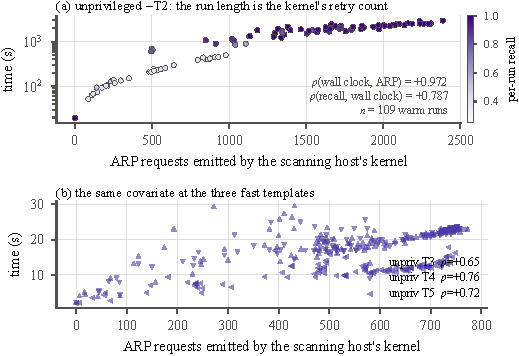
\includegraphics[width=\columnwidth]{figures/fig5_arp_versus_wall_clock}
\caption{\textbf{Unprivileged nmap's run length, and therefore its recall, is
set by the scanning host's kernel rather than by nmap or by the segment.} The
same binary, argv and ten responders produce 0 to 2{,}387 ARP retries for the
244 empty addresses, and the wall clock follows at $\rho=+0.972$; longer runs
are still listening when closed-port resets arrive, which nmap counts as hosts
up. This covariate, not the privilege mechanism, is what refutes H6.}
\label{fig:arp}
\end{figure}

The protocol says the strata exist so ``device sleep cycles and household
network load are sampled rather than avoided'', and lists Wi-Fi contention as a
confound controlled by ``time-of-day strata; passive capture records channel
utilisation''. \textbf{The Wi-Fi covariate is \texttt{not\_applicable} on all
1{,}578 admissible runs}: the 2026-09-06 amendment made the programmable
segment primary, and that segment is five guests on a virtual bridge on the
scanning Mac, which household load, device sleep and channel utilisation cannot
reach.

The measurements agree. The spread across a condition's four warm stratum
medians is 1\,ms for the fixed ablation, 5\,ms for the adaptive default, 9\,ms
for the shared budget, 8\,ms for privileged \texttt{-T5} and 1.5\,s for
privileged \texttt{-T2} on a median of 466\,s. Only one condition shows any
signal under Kruskal--Wallis (exploratory): the adaptive default at
$p=0.0117$, a 5.4\,ms spread across four medians between 0.379 and 0.385\,s.
Unprivileged \texttt{-T2}'s stratum medians span 431 to 1{,}704\,s at
$p=0.57$, which is the ARP covariate and not the clock.
\textbf{Stratification cost the study its seven-day floor and its ten-day
window, and on the primary testbed it sampled the scanning host's own state.}
The secondary physical segment is where it would have mattered, and the paper
cannot claim the strata controlled household contention on this data.

\subsection{Secondary metrics, and sensitivity}
\label{sec:sensitivity}

Jaccard set stability between consecutive blocks is a median 1.000 for every
\netsanity{} condition and every privileged nmap template and \textbf{0.700 for
unprivileged \texttt{-T2}}, the lowest in the study --- the instability
Fig.~\ref{fig:arp} explains. Probes per host discovered, available for
\netsanity{} only since nmap does not report it, is 61.7 adaptive, 62.5 shared,
64.1 fixed. H4 is reported as a discovery comparison rather than the naming
comparison it was meant to be (Section~\ref{sec:notinrecord}):
\texttt{ns full} finds all ten declared responders in 112 of 112 warm runs at
3.05\,s, nmap's broadcast-script equivalent four of ten in 92 of 108 at
28.1\,s.

\paragraph*{The three flagged blocks change nothing} Blocks 36, 74 and 93 ran
partly on battery under records that say otherwise. They are admissible and are
not removed. Running the whole analysis with and without them moves no verdict
in either arm and barely moves a median: the adaptive default 0.382\,s both
ways, the shared budget 1.681 against 1.680\,s, privileged \texttt{-T5}
4.308\,s both ways. The one number that moves is unprivileged \texttt{-T2}'s
warm median, 1{,}446\,s to 1{,}378\,s --- the ARP covariate's spread, not the
battery.

%% Two further generated tables are built by scripts/make_tables.py and are not
%% placed here, because this draft is at the top of the 8--12 page budget the
%% protocol sets: tables/tab_cold_n.tex (cold runs per condition, the numbers in
%% the paragraph below) and tables/tab_precision.tex (precision and found-set
%% size per condition, the numbers in Section V-B). Both are ready to \input if
%% a later cut frees the space.
\paragraph*{The cold arm is small, unbalanced and unpairable} The amendment
predicted about 9.2 cold runs per condition; the realised allocation is 9.4 on
average and \textbf{5 to 15} --- \texttt{ns adaptive} 5, \texttt{ns shared} 7, \texttt{priv T2} 5, \texttt{unpriv T4} 15, because the flush happens
at block start and which condition lands first is whatever the shuffle put
there. \textbf{The two conditions H5 turns on have the two smallest allocations
in the study.} Six of the 52 condition-by-stratum cells hold no cold run at
all, against the amendment's predicted 4.7. And the warm arm's $n\ge30$ per
stratum is about \emph{blocks}: a given condition's warm count per stratum is
thirty minus its cold draws plus whatever the two partial blocks contributed,
which lands between 24 and 31. That is worth a sentence in any paper that
states $n\ge30$ about blocks and is read about observations.


\section{Threats to validity}
\label{sec:threats}

\subsection{What the data will not support, whatever the verdicts say}
\label{sec:notinrecord}

\paragraph*{Anything about RTT dispersion, which is the central mechanism}
That the advantage is proportional to $\qhigh/\qlow$ and vanishes on a
homogeneous segment is the prediction H2 exists to test, and the one this
collection cannot test. \textbf{The testbed holds one dispersion,
$\mathbf{546\times}$ as measured, identical at all seven apparatus commits;
nothing in 1{,}580 runs varies it.} The segment was made programmable precisely
so the dispersion curve could be swept, and the collection swept time of day
instead --- the axis Section~\ref{sec:strata} shows had nothing on it. A claim
that the advantage scales with dispersion is a claim from the simulator, not
from this data.

\paragraph*{Anything about correlated loss} The simulator predicts H5 fails
under bursty loss and names it the regime where the technique is paid for. Nine
of ten responders carry 0.0\% loss and the tenth a flat 15\%; no burst process
was imposed and burstiness was never estimated. The arm where H5 was predicted
to fail hardest is not sampled.

\paragraph*{The cost model, and three of five secondary metrics} The record
carries \texttt{probes\_sent} --- a median of 703 against $Nk=762$ --- and
neither $c$, $r$ nor $t$, so the wave form cannot be fitted and
Section~\ref{sec:vs-sim} prices its disagreement with the simulator without
resolving it. Time to first host and peak in-flight probes are not recorded, so
Little's Law is untested. Energy per scan is not in the schema and could not
have been collected as specified anyway: the protocol asks for
\texttt{powermetrics} on battery with the screen off, and the driver refuses to
start a block unless the host is on AC --- two controls in one protocol that
cannot both be satisfied.

\paragraph*{H4, at all, from this file} H4 carries no test, but its metrics ---
the fraction of hosts given a human-meaningful name, the fraction given a
model, the fraction of randomised-MAC hosts named at all --- are \textbf{not in
the record}: the artifact holds the names, the NDJSON only that the naming
stage ran. Schema~2 was cut to fix exactly this class of gap for the discovery
stage and did not extend it to naming. \textbf{This is the one place the
protocol's own rule --- no number in the paper may exist that cannot be
recomputed from the record --- is not met by the collected file}, and it is
stated rather than worked around.

\paragraph*{Anything outside one machine and one network} One hardware model
(Mac16,8, Apple M4 Pro), one OS build (macOS 26.6.2 / 25G83), one /24, no
Wi-Fi, no IPv6, no routed topology; the secondary physical testbed was never
used for collection, so the external-validity arm the 2026-09-06 amendment
retained is unexercised. The dead-dominated regime
Eqs.~\ref{eq:shared}--\ref{eq:split} assume needs $h\ll N$, which holds on
consumer /24s and fails in a dense VLAN; the simulator locates that boundary at
$h=14$ on a /24 at $c=240$, and this testbed sits at $h=10$. H6 is a
local-segment claim because its mechanism is ARP, which does not cross a
router.

\subsection{Internal and construct validity}

We wrote one of the systems and chose its defaults, and the ordering of every
discretionary choice is recorded so a reviewer can check it. The testbed is an
instrument and not a network: ten responders, five latencies, one loss rate.
``Reliability'' is operationalised throughout as recall, precision and set
stability rather than used as an English word.

\textbf{The capture oracle can miss traffic, in one specific way this paper
relies on.} It is bracketed around the process, so for a condition exiting at
0.35--0.42\,s it closes before a 508\,ms reply can land. That is why
Section~\ref{sec:cache} takes its evidence from the condition whose process
lives 3.08\,s, and why the wire counts in Table~\ref{tab:budget}'s short cold
rows are not the number of replies the segment sent.

\textbf{Recall measured on the warm arm is not a property of the scanner} but
of the scanner plus the neighbour table left by the previous run in the block,
and 1{,}458 of 1{,}580 runs are warm. \textbf{And the comparator's ``best
timing template'' is not a fixed object}: before collection H6's clause meant
``whichever template nmap does best with'', and after collection it selects the
template whose recall is a function of how long the scanning host's kernel made
it wait. It is read as written, because reading it any other way after seeing
the data is the move the protocol exists to prevent.

Two biases we could not remove point in opposite directions and are each on the
order of a millisecond against a 382\,ms median (Section~\ref{sec:independence}).
Three blocks violated the plugged-in control and the record cannot show it, and
one rebuild calibrated five times worse than the others across thirteen runs;
neither moves a verdict
(Sections~\ref{sec:record},~\ref{sec:sensitivity}).

\subsection{Conflict of interest}

Declared in Section~\ref{sec:intro-coi}. Where the author chose between designs
after a pilot had shown which way the result leaned --- the cache-state ruling
of Section~\ref{sec:design} --- the options, their measured costs, the choice
and the name of the person who made it are in the protocol, together with the
commitment that a refutation in the under-sampled arm goes in the abstract.
This paper's abstract is that commitment being kept.

\section{Reproducibility}
\label{sec:repro}

\paragraph*{What was measured} \netsanity{} 0.4.0 at commit \texttt{ad09ed1},
tag \texttt{study/binary-2026-09-12b}, \texttt{sha256} \texttt{b4220600\ldots},
Apple Swift 6.3.3, \texttt{arm64-apple-macosx26.0}; nmap 7.991 from a Homebrew
bottle, \texttt{sha256} \texttt{b522bd2f\ldots}; macOS 26.6.2 build 25G83 on a
Mac16,8. The harness re-hashes both binaries on every run, so the appendix's
numbers and the data's are the same numbers, and both hashes are constant
across all 1{,}580 records.

\paragraph*{What the checksum is for, and what it is not for} \textbf{It is not
a claim that the build is reproducible. It is not.} Two \texttt{swift build -c
release} runs of the same commit, at the same path, on the same machine,
minutes apart, produce binaries of identical size differing in 2{,}684 bytes:
16 in \texttt{LC\_UUID}, 212 in a 16-bit field at 106 sites in
\texttt{\_\_TEXT}, and 2{,}456 inside the ad-hoc code signature that hashes the
pages the other two changed. Building at a \emph{different} path adds 2{,}368
bytes, because the absolute build directory is embedded 212 times. The checksum
is a property of the artifact and of where it was built, not of the source.
What it is for is the question the study needs answered --- \emph{did every
block measure the same binary?} --- answered from the data rather than from a
promise. A reviewer rebuilding from the tag gets a different hash and the same
program.

\paragraph*{How to re-run it} Collection ran unattended from a detached
worktree under a launchd agent, with root from a \texttt{sudoers} entry scoped
to three absolute paths for one user and removed afterwards. The analysis needs
neither the network nor the machine, and regenerates every number and figure
here from the published NDJSON and its stratum sidecar:
\texttt{analysis/strata.py -{}-check}, \texttt{analysis/verify.py} and
\texttt{analysis/run\_analysis.py}, then \texttt{Paper/scripts/make\_figures.py}
and \texttt{make\_tables.py}. The one exception is the artifact-existence
check, which needs the raw stdout, stderr and pcap files that are git-ignored
by design --- a capture is of a network that no longer exists in that state ---
and ship as a release bundle.

\paragraph*{The window survived eight interruptions and the record shows each}
Three battery shutdowns, one reboot, two sleeps and two further power losses,
each costing a rebuild recorded with its calibration, identity check and
frozen-package diff. A host \emph{sleep} degrades the segment without
destroying it, which is worth checking for rather than assuming: after one
five-hour sleep, twenty pings per responder put one responder 10.45\% off
target against a 10\% tolerance and another answering 17 of 20 with an 801\,ms
tail. The sharpest operational lesson is \textbf{hold the host awake before
touching the testbed, the way the driver does before touching a block}: one
rebuild took two and a half hours because the machine idle-slept every one to
two minutes with nothing holding it awake. That is the rebuild whose worst
error is 7.00\%.

\section{Conclusion and future work}
\label{sec:future}

Separating the retransmission budget from the absence-declaration budget makes
a local sweep an order of magnitude faster than the fastest comparator
configuration matching its completeness, with complete distributional
separation. That is not the interesting part. The interesting part is that the
same study refutes two of its own four hypotheses, and that the mechanism
behind both is a single number the authors shipped: a declaration budget of
about 370\,ms on a segment whose slowest host answers at 508\,ms. The theory
states $t\gtrsim\qhigh$ explicitly; the implementation derives $t$ from the
replies it has seen, so where the fast hosts answer first the tail is never
sampled. Per-transmission identity --- the contribution --- buys nothing when
the pending table is emptied before the late reply arrives, and a warm
neighbour table hid that in 1{,}458 of 1{,}580 runs, in a table the
experiment's own block structure filled.

\paragraph*{What this study caused to be built}
\label{sec:engine}
\textbf{\netsanity{} had no privileged engine while this data was collected,
and it has one now because of what this data said.} The privileged BPF engine
--- a layer-2 ARP sweep composed with the existing ICMP sweep so that root can
never find fewer hosts than no-root --- was designed, built and landed
\emph{after} the last block, and is checked from the wire rather than from its
own artifact, because this study established that an artifact's self-report of
its engine is not evidence. \textbf{It appears in no result and no figure here,
and every number in this paper was produced by the single unprivileged engine
that existed during collection.} Measuring it is the next study, and the first
question is whether ARP makes the cold arm's two 500\,ms responders a
non-question.

\paragraph*{The three experiments this one could not run} \emph{Sweep the
dispersion}, the axis the central claim lives on and the one this collection
held fixed. \emph{Impose correlated loss}, where the simulator says the
technique is paid for, which this segment does not have and whose repair ---
buying transmission spacing out of the tail budget's slack --- was not
measured. \emph{Balance the cache arms}: one flush per block put the refutation
in the arm with five observations and removed the pairing the plan depends on,
and 240 blocks would fix both at 143 machine hours against 61.

\paragraph*{Two changes to the system, both implied by results above} Derive
the declaration budget from the segment's observed tail with a floor that does
not depend on having already heard it, so $t\gtrsim\qhigh$ is a property of the
design rather than an accident of which host answered first. And reconsider
per-host adaptation: Section~\ref{sec:ablation} prices it at 13--16\% of the
sweep for no measurable return, on a segment whose single dispersion and
constant per-responder latency are the regime where a well-chosen fixed
interval should win. That is not yet a verdict on adaptation --- but it is the
only number the study has, it points the wrong way for the contribution, and it
is reported here rather than left for a reader to derive.

\begin{thebibliography}{99}
\balance
\footnotesize
\bibitem{jacobson1988} V.~Jacobson, ``Congestion avoidance and control,'' in
\emph{ACM SIGCOMM}, 1988.
\bibitem{karn1987} P.~Karn and C.~Partridge, ``Improving round-trip time
estimates in reliable transport protocols,'' in \emph{ACM SIGCOMM}, 1987.
\bibitem{zmap2013} Z.~Durumeric, E.~Wustrow, and J.~A. Halderman, ``ZMap: Fast
Internet-wide scanning and its security applications,'' in \emph{USENIX
Security}, 2013.
\bibitem{masscan} R.~D. Graham, ``MASSCAN: Mass IP port scanner,''
\url{https://github.com/robertdavidgraham/masscan}, 2013.
\bibitem{nmapbook} G.~Lyon, \emph{Nmap Network Scanning}. Insecure.Com LLC,
2009.
\bibitem{varghese1987} G.~Varghese and T.~Lauck, ``Hashed and hierarchical
timing wheels,'' in \emph{ACM SOSP}, 1987.
\bibitem{grosvenor2015} M.~P. Grosvenor \emph{et al.}, ``Queues don't matter
when you can JUMP them!'' in \emph{USENIX NSDI}, 2015.
\bibitem{marinos2014} I.~Marinos, R.~N.~M. Watson, and M.~Handley, ``Network
stack specialization for performance,'' in \emph{ACM SIGCOMM}, 2014.
\bibitem{rfc6762} S.~Cheshire and M.~Krochmal, ``Multicast DNS,'' RFC 6762,
2013.
\bibitem{rfc6763} S.~Cheshire and M.~Krochmal, ``DNS-based service
discovery,'' RFC 6763, 2013.
\bibitem{upnp} UPnP Forum, ``UPnP device architecture 2.0,'' 2015.
\bibitem{martin2017} J.~Martin \emph{et al.}, ``A study of MAC address
randomization in mobile devices and when it fails,'' \emph{PoPETs},
vol.~2017, no.~4, 2017.
\bibitem{nosek2018} B.~A. Nosek, C.~R. Ebersole, A.~C. DeHaven, and D.~T.
Mellor, ``The preregistration revolution,'' \emph{PNAS}, vol.~115, no.~11,
2018.
\end{thebibliography}

\end{document}
